\pagebreak
\section{Discussion}

\subsection{Summary of Results}
There are several behaviors that are controlled by the model parameters. Generally, only M58 models with type 2 weakening produce aternating faults on both side of the ridge axis. All the models show corrugations. As for faulting patterns in terms of evolution frequency, usually Square root is more dynamic than Sinusoidal than Linear, M58 is more dynamic than M57 than M28.

Following tables are a summery of the model behaviors with respect to different setup parameters.
 

\begin{table}[h]
\begin{small}
\begin{center}
\begin{tabular}{||l|l||l|l||l|l||}
\hline
A & Alternating Fault & C & Corrugation & SL & Shear Topography Low \\
\hline
NA& Not Alternating & SF & Secondary Fault on one side & CB & Cut Back   \\
\hline
DD &  Double Dome  & AM    & Atlantis Massif Shape &  &   \\
\hline
\end{tabular}
\end{center}
\end{small}
\caption{Model behaviors in short.}
\label{Tab1}
\end{table}

Based on the 11 models with M variation, we observed eight first-order behaviors as shown in Table~\hyperref[Tab1]{\ref{Tab1}}. 


\begin{table}[h]
\begin{small}
\begin{center}
\begin{tabular}{|l|p{3.5cm}|p{3.5cm}|p{3.5cm}|}
\hline
\diagbox[width=6em]{Type}{M range}&
M28&M57&M58\\
\hline
Type one &NA; C; SL; SF$_{1500 kyr}$; DD    &NA; C; SF$_{1380 kyr}$; CB$_{330 kyr}$; AM(opposite z)     &    \\
\hline
Type two &    &     &    \\
\hline
\end{tabular}
\end{center}
\end{small}
\caption{Linear functional form.}
\end{table}

\begin{center}
\begin{table}[h!]
\begin{small}
\begin{tabular}{|l|p{3.5cm}|p{3.5cm}|p{3.5cm}|}
\hline
\diagbox[width=6em]{Type}{M range}&
M28&M57&M58\\
\hline
Type one & NA; C; SL; SF$_{995 kyr}$ & NA; C; SL; SF$_{760 kyr;1320 kyr}$; CB$_{520 kyr}$; AM & NA; C; SL; CB$_{510 kyr}$; SF$_{760 kyr;1140 kyr;1990 kyr}$   \\
\hline
Type two &    &NA; C; SL; SF$_{680 kyr}$; CB$_{905 kyr}$     & A$_{450 kyr;600 kyr}$; C(only at low M); CB$_{990 kyr}$   \\
\hline
\end{tabular}
\end{small}
\caption{Sinusoidal functional form.}
\end{table}
\end{center}

\begin{table}[ht]
\begin{small}
\begin{center}
\begin{tabular}{|l|p{3.5cm}|p{3.5cm}|p{3.5cm}|}
\hline
\diagbox[width=6em]{Type}{M range}&
M28&M57&M58\\
\hline
Type one & NA; C; SL; CB$_{205 kyr;330 kyr;1025 kyr}$   &      & NA; C$_{1770 kyr}$(due to shear with dif wave length); SF$_{860 kyr}$(high M); SF$_{1190 kyr}$(low M)(Dog Bone); SF$_{1690 kyr}$    \\
\hline
Type two &    & NA; C; SF$_{435 kyr;1060 kyr}$; CB$_{585 kyr}$; CB$_{735 kyr}$; CB$_{910 kyr}$; CB$_{970 kyr}$    & A$_{550 kyr;920 kyr}$; C; CB$_{400 kyr}$    \\
\hline
\end{tabular}
\end{center}
\end{small}
\caption{Square root functional form.}
\end{table}

Generally, all models forms a median valley that deepens and widens toward the lower M side (Figure~\hyperref[fig_Results1_1]{\ref{fig_Results1_1}}) except the reference model with constant M$=0.8$ (Figure~\hyperref[fig_Results1_3]{\ref{fig_Results1_3}}). The topography oberseved in our models, to the first order, is controlled by the spatial and temporal distributions of faulting and to the second order, results from elastically deformation (e.g. The gradual deepening and widening of the median valley; The bending of the crust at the footwall side of the detatchment fault results in a domal shape of the fault interface as a mechanism for producing the dome shape of OCCs). 

The pattern of the deformation (faulting and elastic deformation) is controlled by the evolving stress in the crust in terms of its distribution and magnitude. The stress evolution is a result of the interaction processes between tectonics and magmatism. Due to constant seafloor spreading, tensional stress orthogonal to the ridge-axis in the crust keeps accummulating. At the same time, along ridge-axis varying diking partially accommodates the stress from far field extension and perturbs the homogeneity state of stress distribution along the ridge-axis. Accumulated stress will be largely released when the tensile or shear failures establish.

Since the model behavior is very complicated. We will focus on the effects being brought by the along ridge-axis variation in diking. Thus, it is worth considering a thought experiment with two end members: One, the along ridge-axis coupling is rigid, so that even along ridge axis variation in M exist, once a fault determined to develop, it will cut through the whole model domain along the ridge-axis(Z-axis) simultaneously. The other end member is that there is totally no coupling along the ridge-axis. So that each slice of crossection profile across the ridge behave separately without being influenced by its neighbour to a extreme that the model behavior is just a combination of 20 pseudo-2D models piled up along ridge-axis with their own M. (IMPORTANT: this suggests the importance and urgence for making clear conclusion and results description for previous pseudo-2D models results. However, one difficulty here is that the characteristic fault offset $\Delta X_{c}$ is different between 2D and 3D models.)

\iffalse
\subsection{Cut Back}\label{Sec_CutBack}

\begin{figure}[h]
  \centering
    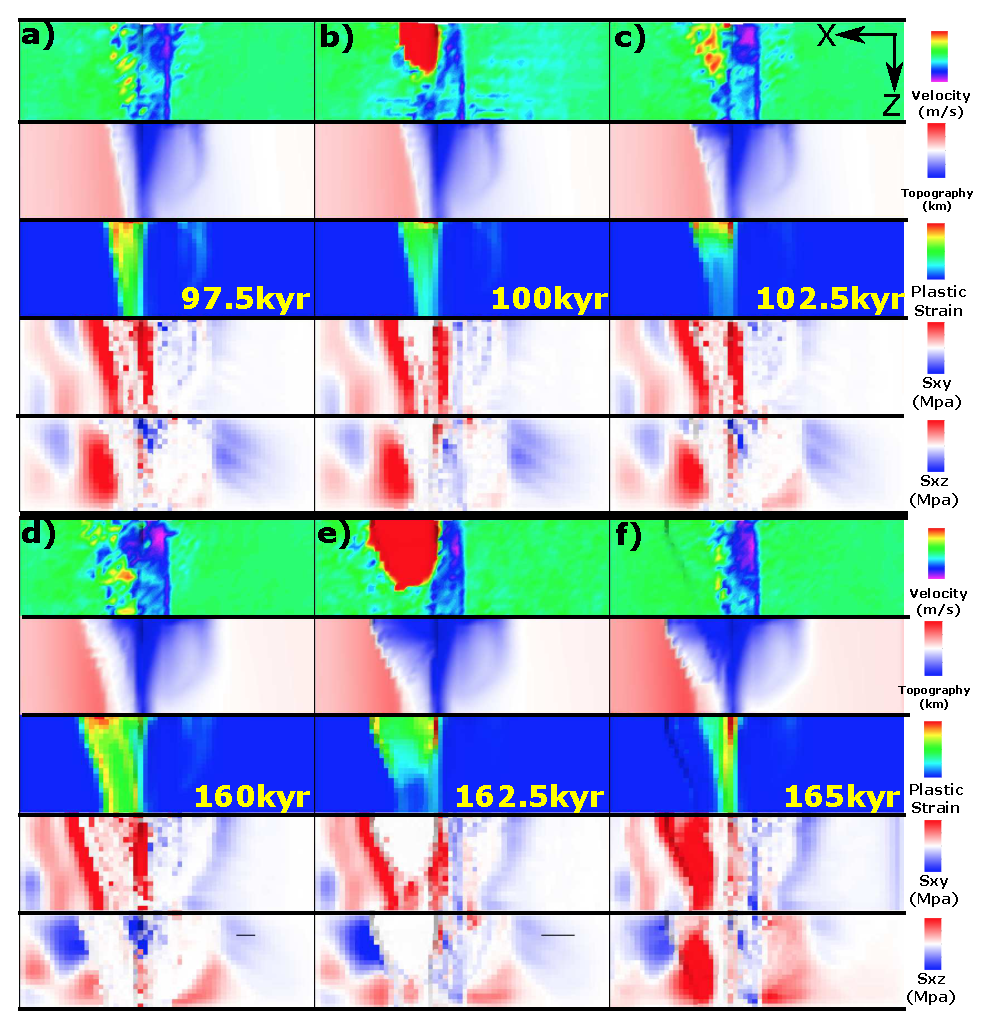
\includegraphics[width=0.8\textwidth]{./Figures/fig_Results4_4_sqrt_cut_back_with_time.eps}
  \caption{M28SqrtT1 (Table~\hyperref[Tab1_1]{\ref{Tab1_1}}). Cut back behaviors in square root functional form model with different time.}
 \label{fig_Results4_4}
\end{figure}   

\begin{figure}[h]
  \centering
    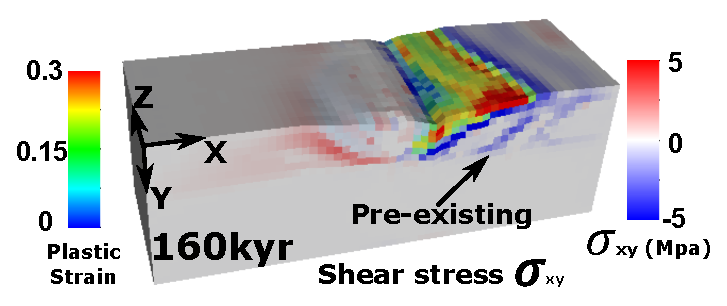
\includegraphics[width=0.6\textwidth]{./Figures/fig_Results4_5_sqrt_cut_back_pre_accummulated_shear_zone.eps}
  \caption{M28SqrtT1 (Table~\hyperref[Tab1_1]{\ref{Tab1_1}}). Square root functional form model at 160kyr. Pre-accummulated shear zone increase the shear force and cut the weak detachment front tip}
 \label{fig_Results4_5}
\end{figure}   

The cut back happens mostly in the square root model. Since the linear model and the square root model have more obvious difference in terms of the cut back behavior, here, we only compare linear and square root. There are several factors contribute to the cut back behavior. First, at the higher M side, the amount of diking for the square root model is ubiquitously larger than that of the linear one (Figure~\hyperref[fig_Results3_1]{\ref{fig_Results3_1}}). This leads to a slower bending detachment at the high M side for the square root model. Second, the totoal length of the ridge segment with M$>0.5$ for the square root model is also longer than that of the linear one (Figure~\hyperref[fig_Results3_1]{\ref{fig_Results3_1}}). This results in that at the low M side, $\sigma_{xz}$ is focused at low Z ajacent to the ridge-axis (Figure~\hyperref[fig_Results4_3_1]{\ref{fig_Results4_3_1}.e}), however for linear is spread out to Z higher than 10. Third, due to higher value of $\frac{dM}{dZ}$ for square root when Z$<5$, the along ridge-axis shear $\sigma_{xz}$ for square root will be accummulating faster, which produces larger strike-slip force to cut the hanging wall at the low M side. Fourth, as observed in the model (Figure~\hyperref[fig_Results4_3_1]{\ref{fig_Results4_3_1}.c}), the parallel to spreading direction offset between breakaways along the ridge-axis is 4km for the square root model compared to 3km for the linear model. This causes the square root model to experience bigger shear stress $\sigma_{xy}$ both immediately beneath and above the fault interface at the low M side (Figure~\hyperref[fig_Results4_3_1]{\ref{fig_Results4_3_1}.d}). Fifth, as shown in Figure~\hyperref[fig_Results4_8]{\ref{fig_Results4_8}}, due to bending of the crust at the footwall side, below the blue neutral plane, $\sigma_{xx}>0$, meaning tensional stress being accummulated as fault develops. The resulting force tends to unbend the bent crust and drag down the connecting surface (the future decoupled hanging wall). All five factors together assist in the decouple of the hanging wall at the low M side as described in detail in the next paragraph.

\begin{figure}[h]
  \centering
    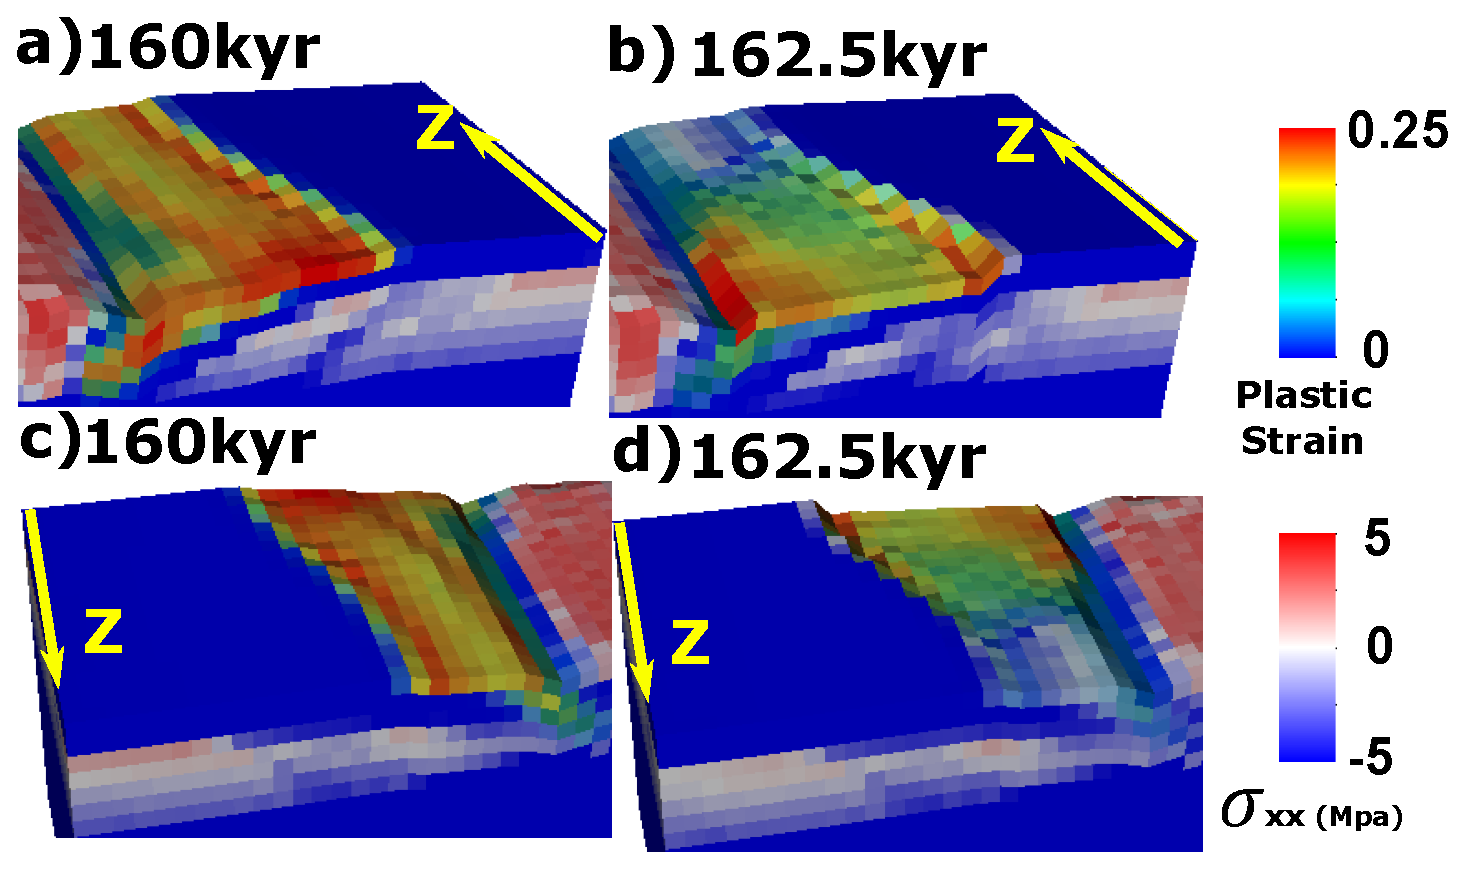
\includegraphics[width=0.6\textwidth]{./Figures/fig_Results4_6_sqrt_cut_back_bending_drop.eps}
  \caption{M28SqrtT1 (Table~\hyperref[Tab1_1]{\ref{Tab1_1}}). Bending stress drop in the crust close to dike due to cut back behavior.}
 \label{fig_Results4_6}
\end{figure}

%(Figure~\hyperref[fig_Results4_6]{\ref{fig_Results4_6}})reveals that
In the Figure~\hyperref[fig_Results4_4]{\ref{fig_Results4_4}}, the hanging wall rebounds backwards to the dike in a high velocity (Figure~\hyperref[fig_Results4_4]{\ref{fig_Results4_4}.b,e (velocity)}) accompanied with a sudden topography drop (Figure~\hyperref[fig_Results4_4]{\ref{fig_Results4_4}.b) compared to c); d) compared to e) (in the second row)}). This behavior is triggered when the front tip of the weak detachment extends further away from the ridge-axis and reaches a pre-accummulated shear zone (Figure~\hyperref[fig_Results4_5]{\ref{fig_Results4_5}}). The pre-accummulated shear zone adds extra shear force to the weak (Figure~\hyperref[fig_Results4_4]{\ref{fig_Results4_4}}.d(third row: plastic strain)) as well as shear stresses accummulated (Figure~\hyperref[fig_Results4_4]{\ref{fig_Results4_4}.d}(fourth and fifth row: $\sigma_{xy}$ and $\sigma_{xz}$)) fault interface and together with the five factors mentioned in the previous paragraph result in the cut back behavior. The cut back produces a continuous high angle fault scarp with a relief of $\sim 1km$ aligns to the initial breakaway and extends for about 20 kilometer in length (Figure~\hyperref[fig_Results4_4]{\ref{fig_Results4_4}.e (second row: topography)}). Its distance to the ridge-axis varies along the Z-axis and this result can be used to indicate the magma supply variation in the nature. \add[XT]{To be discussed in observation comparison section. as a reminder}

During the cut back process, the tensional bending stress are released at the low M side ($0<$Z$<7$) in the left tip of the bended crust (Figure~\hyperref[fig_Results4_6]{\ref{fig_Results4_6}.a compared to b}), however, in the higher M side, the tensional bending stress keeps accummulating due to the far field extension (Figure~\hyperref[fig_Results4_6]{\ref{fig_Results4_6}.c compared to d}). This behavior assists in the decouple between low M and high M side hanging walls. 

Once the cut back happens at 162.5kyr, the $\sigma_{xy}$, $\sigma_{xz}$ and $\sigma_{xx}$ are released (Figure~\hyperref[fig_Results4_4]{\ref{fig_Results4_4}.e (fourth and fifth row: $\sigma_{xy}$ and $\sigma_{xz}$)}). The plastic strain near the ridge-axis at low M side reaches a maximum of $\sim$0.9 (Figure~\hyperref[fig_Results4_4]{\ref{fig_Results4_4}.e (third row: plastic strain)}) compared to $\sim$0.3 before and after. This is due to the sudden backward motion squeezes the end element of the hanging wall near the ridge-axis and later be released by the continuous extension.

After the cut back, the termination of the detachment recedes backwards for about 7 kilometer towards the ridge-axis (Figure~\hyperref[fig_Results4_4]{\ref{fig_Results4_4}.f (third row: plastic strain)}) (termination fronts are always consistent with tension stresses in $\sigma_{xx}$ and $\sigma_{zz}$ as well as with plastic strain front(due to healing, high plastic strain region corresponds only to region with continuously deformation) (Figure~\hyperref[fig_Results4_3_1]{\ref{fig_Results4_3_1}} and Figure~\hyperref[fig_Results4_3_2]{\ref{fig_Results4_3_2}})). This behavior helps maintain a high angle normal fault. Different from the linear and sinusoidal models that the detachments at the low M side will rotate to a very low angle, square root model doesn't. In addition, $\sigma_{xy}$ and $\sigma_{xz}$ soon fill in the area between cut back created fault scarp and the new termination (Figure~\hyperref[fig_Results4_4]{\ref{fig_Results4_4}.f (fourth and fifth row: $\sigma_{xy}$ and $\sigma_{xz}$)} because $\sigma_{xy}$ always accummulates immediately beneath the normal fault interface and the red $\sigma_{xz}$ left to the new termination is due to the along ridge-axis variatioin in the rate of fault slip (low M side larger).  

\begin{figure}[h]
  \centering
    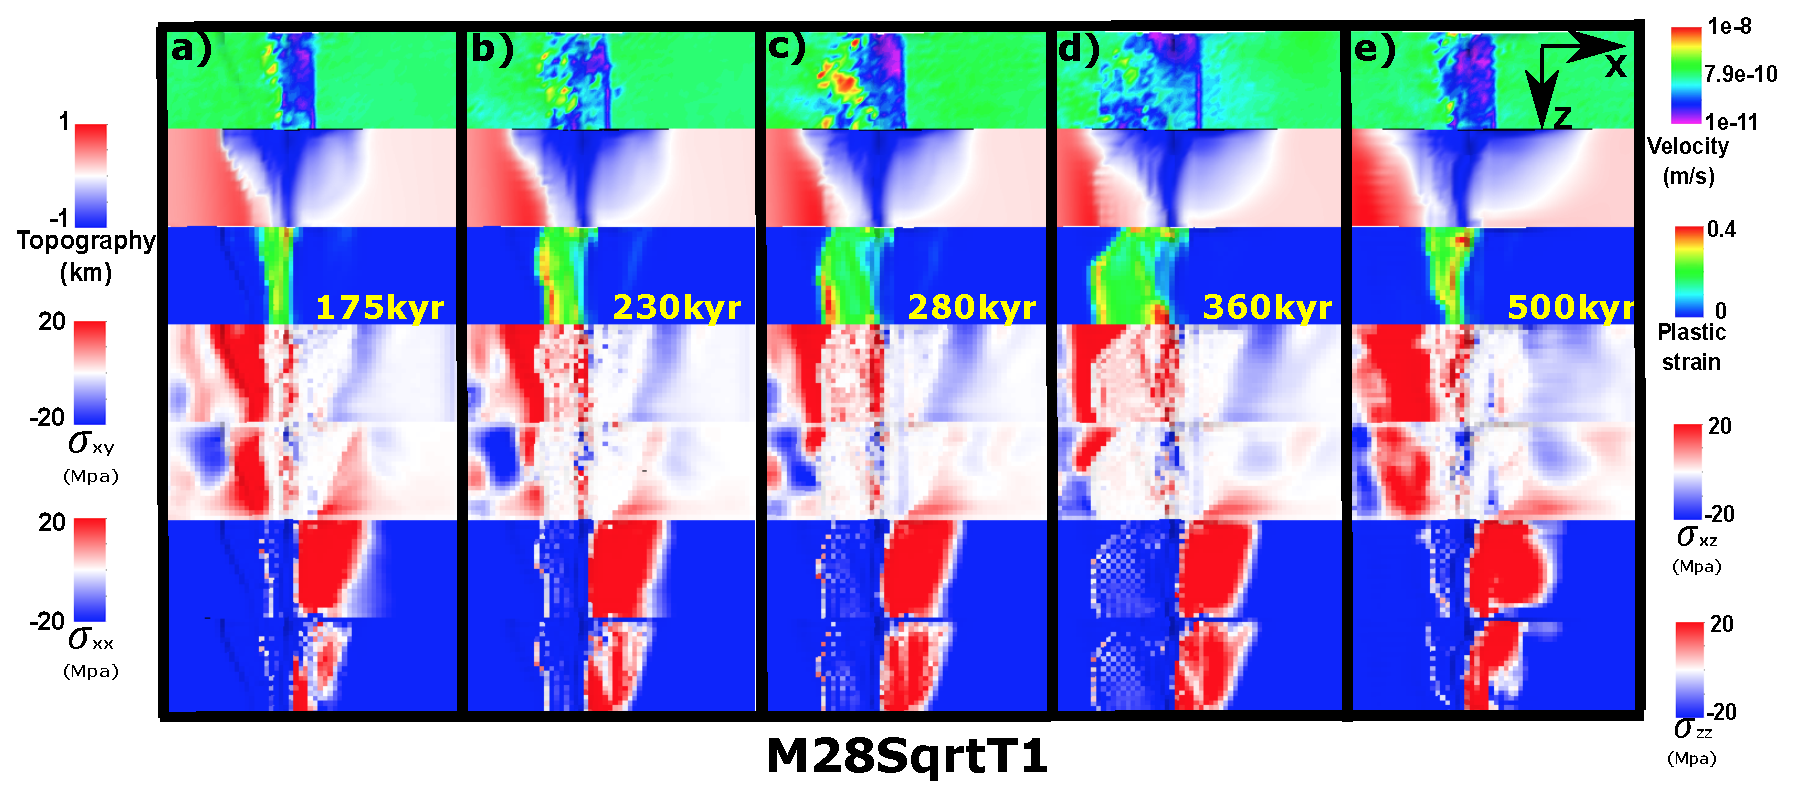
\includegraphics[width=1.0\textwidth]{./Figures/fig_Results4_9_sqrt_cut_back_new_fault_chase.eps}
  \caption{M28SqrtT1 (Table~\hyperref[Tab1_1]{\ref{Tab1_1}}). New fault front chase after initial abandoned breakaway.}
 \label{fig_Results4_9}
\end{figure}

There is one phenomenon very interesting and counter-intuitive that worth describing here. After the cut back, and termination retreat, the evolution of the detachment fronts is opposite to initiall or to the general behavior in the linear and sinusoidal models. The termination front at the high M side extends faster and further after the cut back (Figure~\hyperref[fig_Results4_9]{\ref{fig_Results4_9}}). This is partly related to the unbending decouple phenomenon we described ealier that the tensional stress are released at the low M side but continues to accummulate in the high M side during the cut back unbending in the low M side. Since the tensional stress is released in the low M side, it needs time to accummulate to where it was and then start from there to drag the new near ridge-axis fault away from the ridge-axis while at the high M side the increasing tensional stress will directly lead to a fast extending fault front. Thus create the behavior. \add[XT]{One question is, how to explain that the fault front is moving much faster than the initial abandoned breakaway? New fault front soon reach the old breakaway.} This phenomenon is largely responsible for the corrugations observed. It create a ``X'' shape ``scan'' that first ``scan'' the topography with faster low M side (Figure~\hyperref[fig_Results4_4]{\ref{fig_Results4_4}.d and e}) and then with faster high M side (Figure~\hyperref[fig_Results4_9]{\ref{fig_Results4_9}.c and d}). This results in curved terminations with hundreds to several kilometers wavelengths that directly create parallel to spreading direction corrugations.    

\begin{figure}[h]
  \centering
    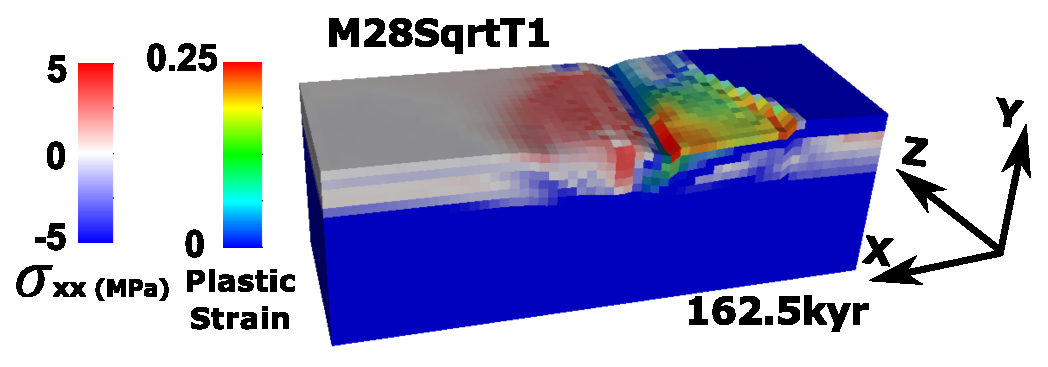
\includegraphics[width=0.6\textwidth]{./Figures/fig_Results4_7_sqrt_cut_back_conjugate_Sxx.eps}
  \caption{M28SqrtT1 (Table~\hyperref[Tab1_1]{\ref{Tab1_1}}). Higher $\sigma_{xx}$ in the median valley of conjugate plate at low M side. }
 \label{fig_Results4_7}
\end{figure}

In addition, the higher $\sigma_{xx}$ in the median valley of conjugate plate at low M side (Figure~\hyperref[fig_Results4_7]{\ref{fig_Results4_7}}) is due to the brittle crust is thinnest at the median valley, thus when same amount of force propagates from far field extension to the center median valley, the stress will increases.    
\fi


\subsection{Fault Alternation}

\subsubsection{Trade-off between bending and weakening}

\begin{figure}[h]
 \centering
  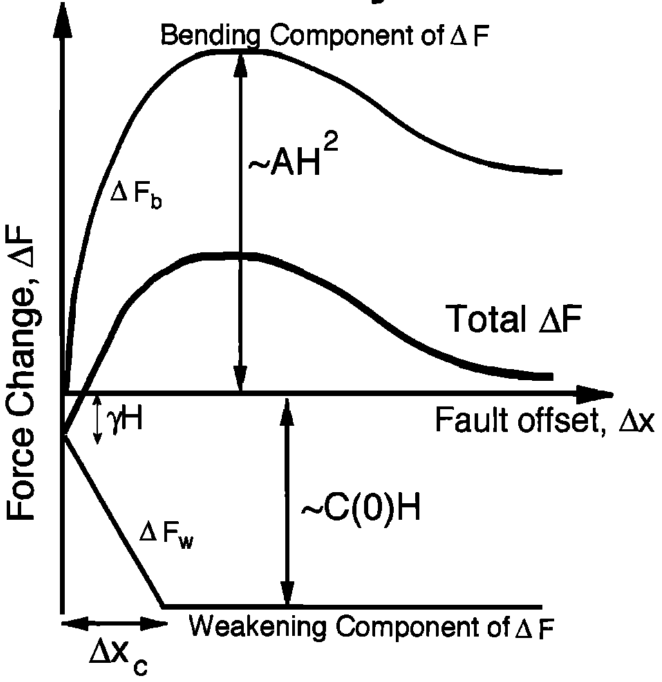
\includegraphics[width=0.45\textwidth]{./Figures/fig_Results_Weakening_1_tradeOff_bend_weak.png}
 \caption{Trade-off between change in bending force $\Delta F_{b}$ and weakening in the fault interface $\Delta F_{w}$. H is the thickness of the brittle crust and $\gamma$ is the size of initial weak perturbation and A defines the maximum bending force change. (For more details, please refer to \citep{Lavier2000})}
 \label{fig_Results_Weakening_1}
\end{figure}

Before we move on to each of the pairs, the framework studied by \citep{Lavier2000} needs to be mentioned here for better understanding the model behaviors observed in our model results. There is a trade-off between change in bending force $\Delta F_{b}$ as a function of fault offset $\Delta X$ and force change $\Delta F_{w}$ as a function of  $\Delta X$ due to strain weakening. As described in \citep{Lavier2000}, higher characteristic fault offset ($\Delta X_{c}$) or slower strain weakening results in multiple faults rather than only one fault lasting. Whether conjugate fault and even multiple faults can be produced depends on the local stress condition. The strength weakening of the existed fault combines with how much bending force resists the fault to keep offseting play a major role in determining the stress state at the other areas. As the sea-floor keeps spreading and  $\Delta X$ increasing, the change in bending force $\Delta F_{b}$ increases and the strength at the fault interface decreases due to weakenging $\Delta F_{w}$ (Figure~\hyperref[fig_Results_Weakening_1]{\ref{fig_Results_Weakening_1}}). If the net force change $\Delta F = \Delta F_{b}+ \Delta F_{w}$ is positive, it means that it is getting harder and harder to maintain the existing fault and stress will begin to accummulate at the other areas which eventually break another fault. $\Delta F_{b}$ initially increases fast with respect to $\Delta X$ and then when the breakaway bends over, it reaches its peak value and begin to decreases a little and maintains at a constant value. If the strain weakenging is fast enough that the net effect force $\Delta F$ is always negative, then most of the stress will be released by the existing fault and thus no conjugate or multiple faults will be created. 

Our model results verify this analysis that only Type two weakening (slower weakening with higher $\Delta X_{c}$) can produce an alternating normal fault on the conjugate plate.

Based on the previous experience in pseudo-2D models and \citep{Lavier2000},  when M$>0.5$, the frequency of normal faulting alternation is higher for higher characteristic fault offset ($\Delta X_{c}$) of Type two weakening compared to Type one weakening. However, for the reference model two, M88ConT2 (Table~\hyperref[Tab1_1]{\ref{Tab1_1}}), interesting enough, when comparing pseudo-2D and 3D models with Type two weakening under case of M$=0.8$, even though the 3D Model has a larger $\Delta X_{c}$ of 1km than that of pseudo-2D model of 0.5kmr, the 3D model M88ConT2 has a lower frequency of faulting alternation. Since M is constant 0.8 along the ridge-axis, the effect of along ridge couplingthat resists alternation need not be considered. One possibility is that the resisting bending force increase in a higher rate than linear with respect to increasing the length of the ridge segment (Z$_{max}$ km).  
\subsubsection{Alternating on conjugate plate}

The fault alternation behavior observed in pseudo-2D models in cases M$>0.5$ is much more complicated in 3D models. The results shows that only Type two weakening with M58 will result in a alternating faulting pattern. \add[XT]{integrate the area of M$>0.5$ with respect to Z to see if there is any quantatative analysis available.}

\subsubsection{Secondary near-axis normal fault}

The secondary near axis high angle normal fault is another common observation of the models. As shown in Figure~\ref{fig_Results1_1}, at the ridge axis with M$>0.5$ (i.e. Z$>10$), the existing normal fault will be pushed away from the ridge-axis due to excessive diking, as its mechanism has been mentioned in the introduction chapter, another new near axis normal fault is created at around 650kyr. As it evolve, the initial detachment fault become inactive (the transparant view of plastic strain shown in the rigth corner inset of time 880kyr). This secondary fault creates another dome and its composition is more likely to be volcanic rather than ultramafic, however, as is evolve, if it can last long, lower crust and upper mantle material can be exhumed to the surface. The composition of the domes observed at Kane magamullions is similar to this mechanism that ultramafic Babel dome is on the West and crustal inside-corner high on the East.    

\subsubsection{Effect of along ridge-axis coupling}
The along ridge-axis coupling allowed the normal fault at the high M side (M$>0.5$) to last for a long time and become a detachment that can produce a OCC. This behavior is different from previous 2D studies that only M=$0.3\sim0.5$ can make OCCs and it also provides an alternative explanation for reconciling the gap between 2D model and observation described in \citep{Olive2010}. Instead of magma injecting below brittle dutile transition, even injecting in the crust, due to along ridge coupling, model can still create OCC for high magma supply. Find the observation evidence for high M OCC from refs of Olive2010. As mentioned in the abstract of Olive2010, ref4-11 show a spectrum of magma supply.

\subsection{Corrugations}
There are two contributing factors, for one, trans-extenstional stresses are created due to offset of the breakaway as well as the variation in fault displacements along the ridge axis; for the other, the variation of the positions of the terminations of the detachment faults along the ridge-axis creates anastomosing faults that is mentioned in \citep{Smith2014}. This anastomosing faulting behavior is largely responsible for corrugations in our models.      

The stress at the tips of the breakaways is generally tensional in both parallel and orthogonal directions to the ridge-axis. (Figure~\hyperref[fig_Results4_3_1]{\ref{fig_Results4_3_1}.f,g})

\subsubsection{Wavelength of corrugations}

\subsection{Influence of healing}

\subsection{Comparing model results with nature observation}

\subsubsection{Cut back at 13$\degree$N Mid-Atlantic Ridge (M28SqrtT1)}

\begin{figure}[h]
 \centering
  \includegraphics[width=1.0\textwidth]{./Figures/fig_Discussion_Observation_1_13N_MAR_CutBack.eps}
 \caption{Comparing nature observation at 13$\degree$N Mid-Atlantic Ridge to the Cut back behavior of model M28SqrtT1. The model topography is a mirror symetric flip according to the dash line, it reveals the case of M varies in a square root functional form from 0.2 to 0.8 to 0.2. For discussion on cut back formation mechanism, please refer to Section~\hyperref[Sec_CutBack]{\ref{Sec_CutBack}}. The bathymetry is from GeoMapApp \citep{Ryan2009}.}
 \label{fig_Discussion_Observation_1}
\end{figure}

The cut back behavior in M28SqrtT1 model creates a fault scarp of $\sim$1km in relief, 40km in length along the Z axis. Note that the fault scarp corresponds to initial formed breakaway. The topography at 13$\degree$N Mid-Atlantic Ridge also has a fault scarp with very similar geometry with $\sim$1km in relief. Due to the variation in diking along the ridge-axis, a sandglass shape of median valley is also produced in the model where the narrowest center corresponds to the region with high magma supply (M=$0.8$). This sandglass shape is also frequently observed in the nature along the Mid-Atlantic Ridges.
 
\subsubsection{Double dome at 23$\degree$N Mid-Atlantic Ridge (Kane Megamullions) (Several models)}

\begin{figure}[h]
 \centering
  \includegraphics[width=1.0\textwidth]{./Figures/fig_Discussion_Observation_1_13N_MAR_CutBack.eps}
 \caption{Comparing nature observation at 13$\degree$N Mid-Atlantic Ridge to the Cut back behavior of model M28SqrtT1. The model topography is a mirror symetric flip according to the dash line, it reveals the case of M varies in a square root functional form from 0.2 to 0.8 to 0.2. For discussion on cut back formation mechanism, please refer to Section~\hyperref[Sec_CutBack]{\ref{Sec_CutBack}}.}
 \label{fig_Discussion_Observation_1}
\end{figure}

\subsubsection{Atlantis Massif Shape at 30$\degree$N Mid-Atlantic Ridge ()}
\subsubsection{Shear low}
\subsubsection{Corrugations}


%\subsection{Parallel computing efficiency}

\subsection{Model Limitation}

\subsubsection{Fixed thermal structure effects and justification}
Thermal conduction rate for $\kappa=6mm^{2}/s$ material is 1.8e5 km/Myr, four magnitude faster compared to spreading rate of 2.5km/Myr.

\subsection{Recommendation for Future Research}
